\documentclass{article}
\usepackage{graphicx} % Required for inserting images
\usepackage{amssymb}
\usepackage{amsmath}
\usepackage{float}
\usepackage{multirow}
\usepackage{booktabs}
\usepackage{array}
\usepackage{subcaption}
\usepackage{listings}
\usepackage{xcolor}
\usepackage{eurosym}
\usepackage{enumitem}
\usepackage{hyperref}
\usepackage[backend=biber,style=alphabetic]{biblatex}
\addbibresource{references.bib}
\lstset{
    language=Python,
    basicstyle=\ttfamily\small,
    keywordstyle=\color{blue},
    commentstyle=\color{gray},
    stringstyle=\color{red},
    showstringspaces=false,
    frame=single,
    breaklines=true
}
\usepackage[margin=2.5cm]{geometry}
\setlength{\parindent}{0pt}


\graphicspath{{./images}}

\title{ELEC70103 Machine Intelligence for Finance}
\author{Adam Ali (aa5222@ic.ac.uk, CID 02252150}
\date{January 2026}

\begin{document}

\clearpage
\section{Graphs in Finance - B}

Markov chains are a staple of systematic trading strategies. They are a backbone within Quantitive Research for predicting future states based on what has been seen historically. Together with \textbf{Vishesh Mongia - CID X}, we model daily equity returns as belonging to one of several states. Movement from one state to another can be represented as a transition on a directed graph. For example, if a stock rises on one day, it is often followed by a fall on the next, since markets typically exhibit some mean reverting behaviour. \\
%TODO FIX THE ABSTRACT

This setting naturally admits a graph representation because the problem is fundamentally about transitions between states. The graph is useful because it makes temporal dependence interpretable: for example, we can visualize persistence in one state, reversal between states, and other asymmetry in price movement patterns. \\ 

The study also benefits from graph optimisation because the graph can be used for decision-making. A trading strategy can be constructed by using the transition probabilities to estimate the expected next-day return conditional on the current state.\\

In our research, we use Claude Opus 4.6 exclusively, due to its powerful reasoning and coding abilities.

\subsection{Prompt 1 - Simple Markov Chain}
\subsubsection{Prompt}
``I am designing a finance study based on graph representations and graph optimizations. My idea is to model daily stock returns as a Markov chain, where each node is a discrete state and each directed edge is the probability of moving from one return state to another tomorrow. I want to build and test a trading strategy from this.  Please help me refine this framework, specifically:

\begin{enumerate}
    \item Suggest a good financial setting for this idea: single stocks or ETF's?
    \item Propose sensible ways to discretize the nodes in the graph
    \item Identify weaknesses of this approach, including non-stationarity, sparse transistions, and transaction costs. 
    \item Suggest how I should split the data into training and testing sests and evluate the strategy out of sample''
\end{enumerate}

This prompt is strong because it does not ask the LLM to do the whole assignment blindly. Instead, it directs the model to improve specific parts of the framework. \\

\subsubsection{Response}

\begin{itemize}
    \item I would recommend training the Markov model on a broad equity index like the S\&P 500 (SPX) rather than on individual stocks or sector ETFs. 
    \item You can bucket daily returns into discrete intervals - e.g. large negative, small negative, small positive, large positive, and count the transitions between bins, giving 4 bins.
    \item Non-stationarity. The Markov property assumes the transition probabilities are constant over time. In reality, the structure of market regimes evolves — the dynamics of a post-2008 QE-driven market are different from a pre-crisis environment. A model trained on 2010–2018 implicitly averages over these sub-periods. Mitigation: use a training window long enough to span multiple market cycles (bull, correction, crisis) so the model sees a representative sample of transitions, but not so long that very old data dominates.
    \item Training set: 2010-01-01 to 2018-12-31 (~9 years). This window includes the 2010–11 Euro crisis, the steady 2012–14 bull, the 2015–16 China volatility, the ultra-calm 2017, the Feb 2018 VIX spike, and the Q4 2018 sell off. 
    \item Evaluation metrics: Annualised Sharpe ratio for the strategy vs. buy-and-hold on each stock. Cumulative return comparison.
\end{itemize}

\subsubsection{Evaluation}
Using this, we can formalize the first-order Markov chain with K states as a directed weighted graph $G = (V, E, w)$:


\begin{itemize}
    \item Vertices $V = \{s_1, \dots, s_K\}$: one node per discretised return state.
    \item Edge weights $w(s_i, s_j) = \hat{p}_{ij}$: the maximum-likelihood estimate of $P(S_{t+1} = s_j \mid S_t = s_i)$, computed as:
\end{itemize}

$$\hat{p}_{ij} = \frac{n_{ij}}{\sum_{k=1}^{K} n_{ik}}$$


where $n_{ij}$ = number of observed transitions from state $i$ to state $j$ in the training data.
Given the current state $s_i$, compute the conditional expected return for tomorrow:
\[
\hat{\mu}_i = \sum_{j=1}^{K} \hat{p}_{ij} \cdot \bar{r}_j
\]
where $\bar{r}_j$ is the average realised return within state $j$. This represents the expected one-day return conditional on being in state $s_i$ today. Now we can define a simple rule for our trading strategy:

\[
\text{Position}_{t+1} =
\begin{cases}
+1 & \text{if } \hat{\mu}_{s_t} > 0 \\
0  & \text{if } \hat{\mu}_{s_t} = 0 \\
-1 & \text{if } \hat{\mu}_{s_t} < 0
\end{cases}
\]

We want to examine how the market will evolve, multiple steps into the future. Using the $n$-step transition matrix $\mathbf{P}^n$, define:
\[
\hat{\mu}_i^{(n)} = \sum_{j=1}^{K} [\mathbf{P}^n]_{ij} \cdot \bar{r}_j
\]

Here, $[\mathbf{P}^n]_{ij}$ is the probability of transitioning from state $i$ to state $j$ in $n$ steps. Finally, we employ the Markov Decision Process (MDP) strategy. The algorithm finds the policy that maximises the minimises the discounted long-run cumulative reward using the Bellman equation:

\[
V(s_i) = \max_{a \in \{-1,0,1\}} \left[ a \cdot \left( \mathbf{P}_i \cdot \bar{\mathbf{r}} \right) + \gamma \sum_{j} \hat{p}_{ij} \, V(s_j) \right]
\]

By solving by iteration, the MDP accounts for multi-step consequences. In our model, we ignore transaction costs. This format does not penalize frequent position switching. 

To determine how many nodes we should use in our chain, we carry out a small hyper parameter tuning on the validation set. This returns K as 7. We plot the transition matrix to explore these regime shifts more closely. The MDP strategy outperformed the Buy \& Hold over the out-of-sample testing period in 2018, from a pure returns point of view (figure 25). The Sharpe ratio was also higher for the MDP (0.679 vs -0.429). 

\begin{figure}
    \centering
    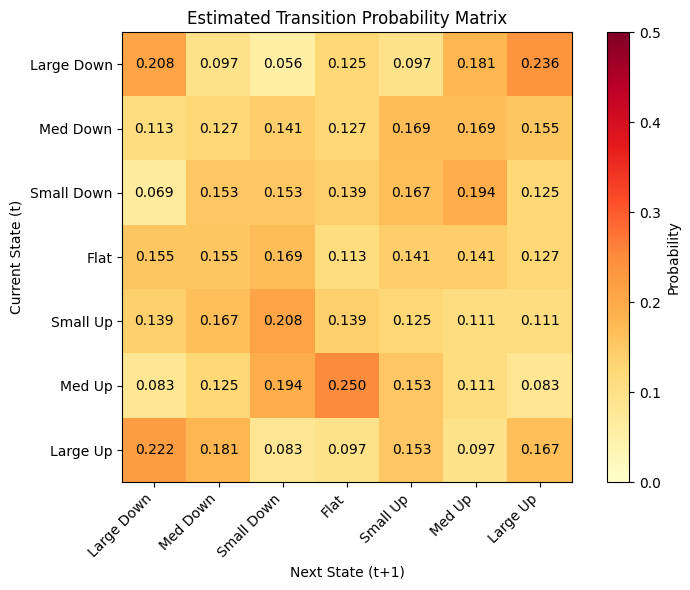
\includegraphics[width=0.75\linewidth]{images/simpleTransition.png}
    \caption{Transition matrix for 7 states}
    \label{fig:placeholder}
\end{figure}

\begin{figure}[h!]
    \centering
    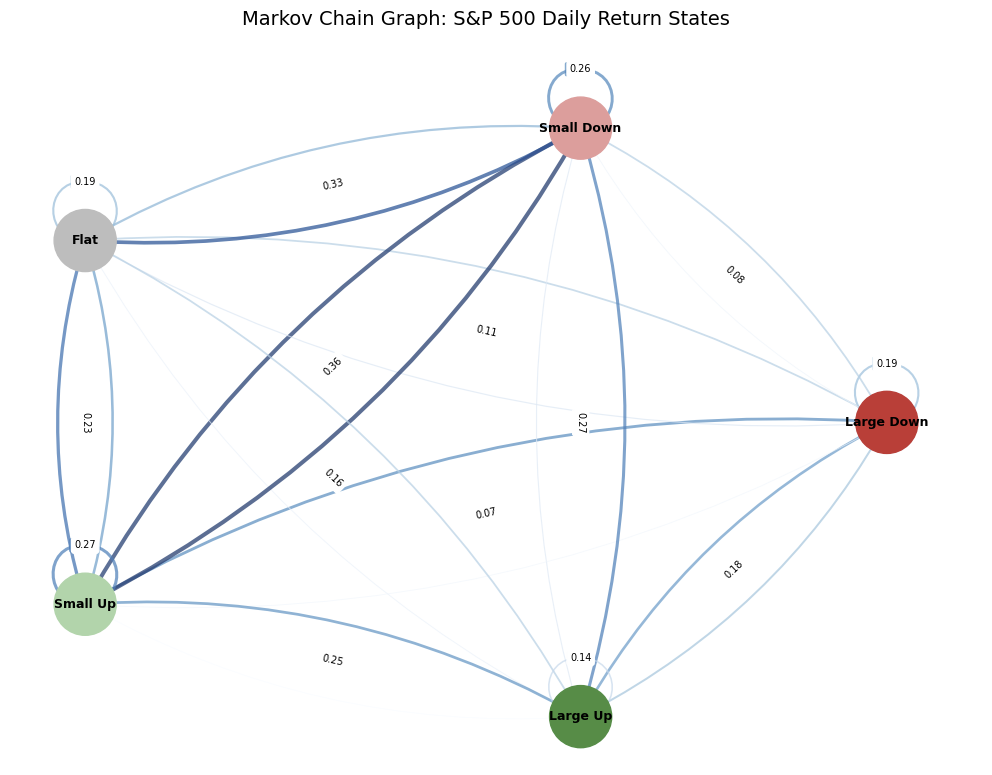
\includegraphics[width=0.75\linewidth]{images/simpleMarkov.png}
    \caption{Simple Markov chain with 4 states}
    \label{fig:placeholder}
\end{figure}

\begin{figure}
    \centering
    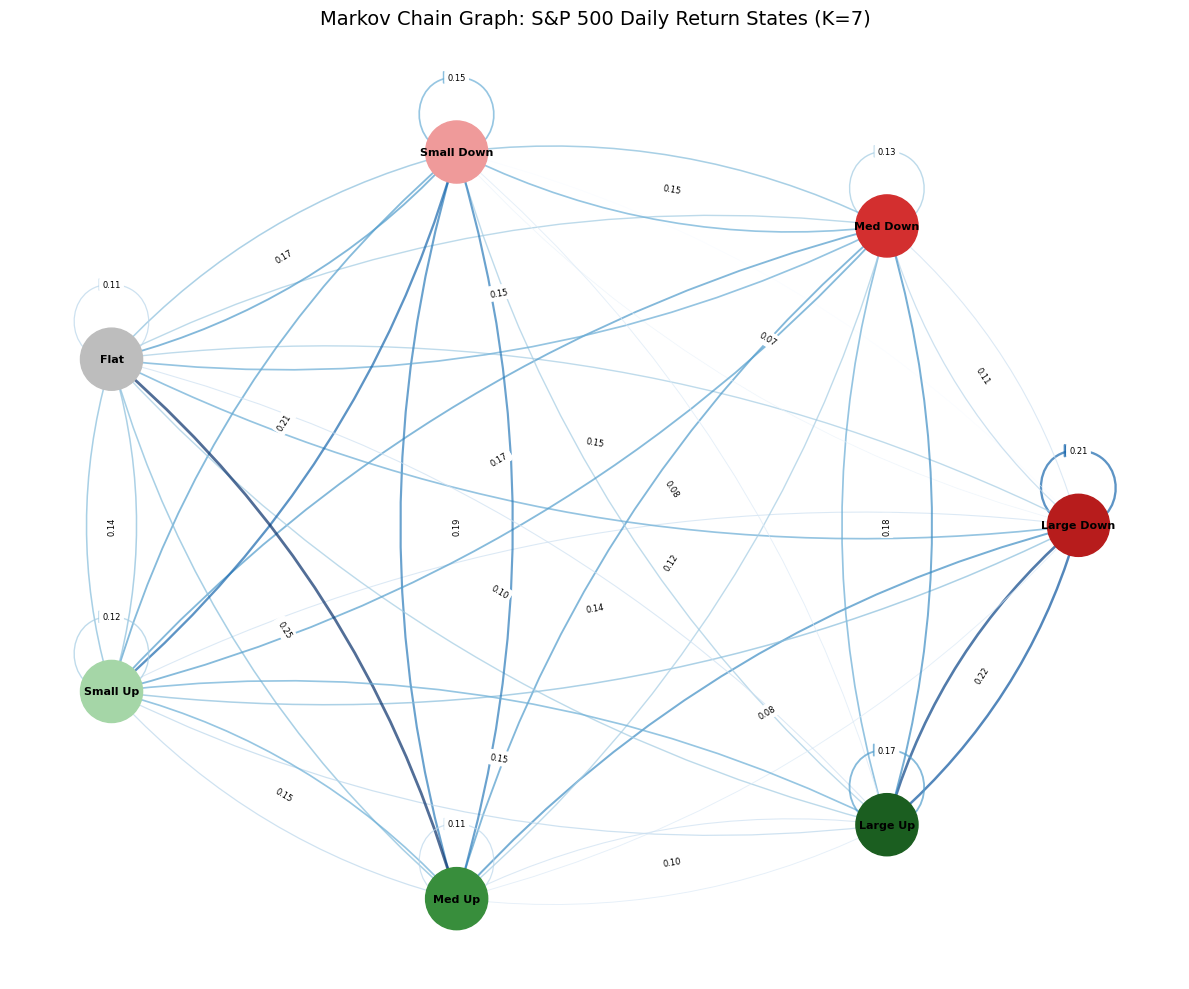
\includegraphics[width=0.75\linewidth]{images/simpleMarkov7.png}
    \caption{Optimized graph with k=7 states}
    \label{fig:placeholder}
\end{figure}

\begin{figure}
    \centering
    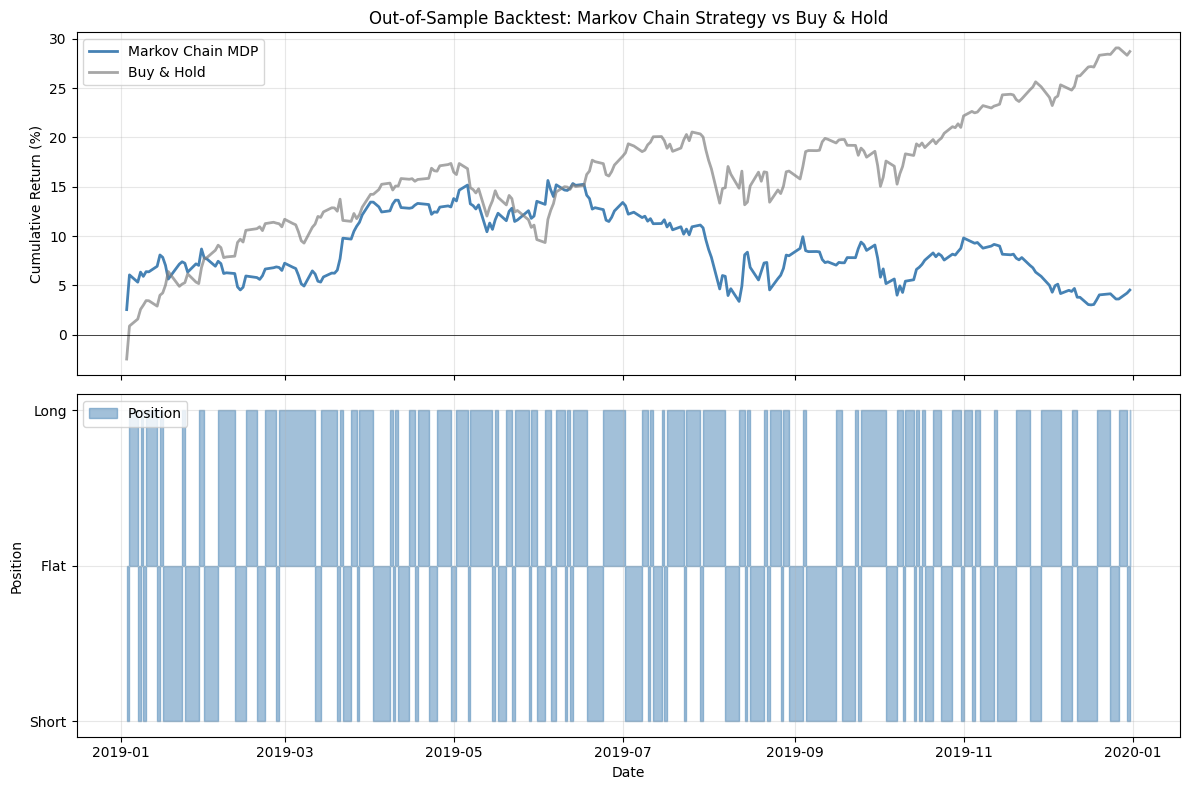
\includegraphics[width=0.85\linewidth]{images/simpleMarkovReturnsGraph.png}
    \caption{MDP Strategy vs Buy \& Hold, as well as position direction}
    \label{fig:placeholder}
\end{figure}
\clearpage
\subsection{Prompt 2 - Hidden Markov Model }
A concern was that some of the transition probabilities in figure 22 where rather noisy. For example, the most probable next move from a large upswing was a large downswing at 22.2\% of the time! This seemed counter-intuitive.\\

\subsubsection{Prompt}
``Are there better ways to discretize the node states, rather than just using return percentage groupings?"

\subsubsection{Response}
``The core issue is that the bin edges are arbitrary and context-blind. A $-1.5\%$ day means something very different in a low-volatility environment (a major move) versus a high-volatility crisis (a quiet day). By grouping purely on return magnitude, you mix fundamentally different market conditions into the same node. You also lose all information about the volatility regime: two days with identical $+0.3\%$ returns get the same label regardless of whether surrounding volatility was $8\%$ annualised or $40\%$ annualised.\\

Additionally, the bin widths interact badly with non-stationarity. If you set your edges based on what looks reasonable for 2012–2014 (a calm period), too many crisis-period days pile into the extreme bins. If you calibrate to include 2008-style moves, the extreme bins are nearly empty during normal markets and the transition matrix becomes sparse.

\begin{itemize}
    \item Alternative 1: Volatility-Normalized Bins. Z-score each of the day's return relative to a rolling volatility estimate. 
    \item Alternative 2: Clustering K-Means/GMM). You can cluster return observations using K-means of Gaussian Mixture Models. This lets the data determine the cluster centres rather than imposing fixed percentage thresholds. 
    \item Alternative 3: Hidden Markov Model. A simple Markov chain assumes that the market's state is directly observable. A HMM acknowledges that the true market state is hidden, and can only be inferred from multiple observable signals. Within a state k, it assumes we generate returns according to a Normal distribution with mean $\mu_k$ and volatility $\sigma_k$. ''
    
\end{itemize}

\subsubsection{Evaluation}
\begin{figure}[h!]
    \centering
    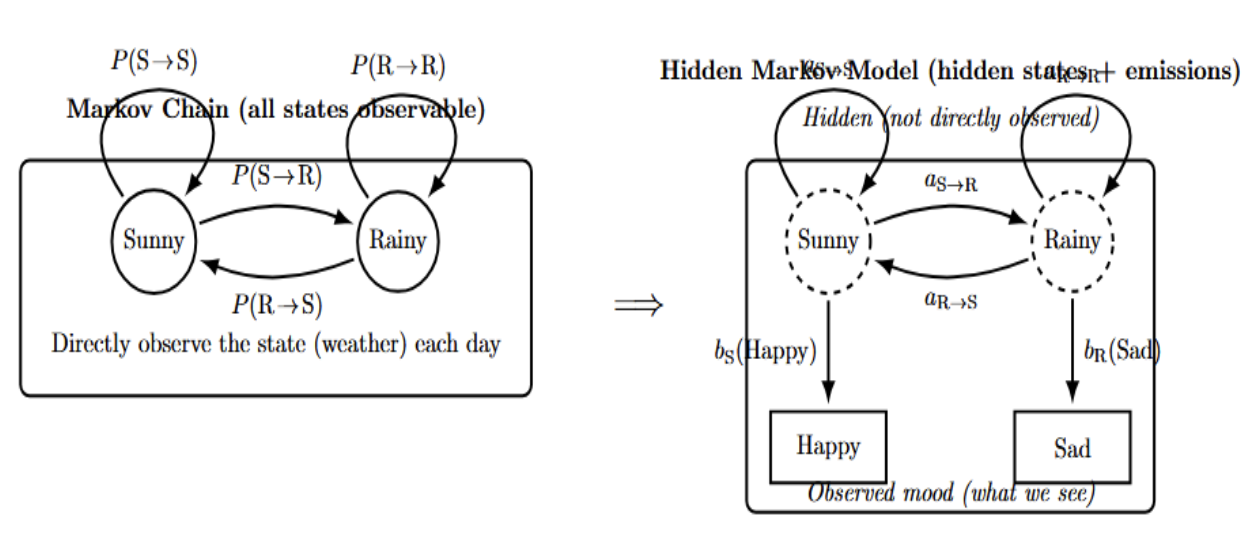
\includegraphics[width=0.85\linewidth]{images/Image_2.png}
    \caption{Weather Example: Simple Markov vs HMM}
    \label{fig:placeholder}
\end{figure}


The HMM suggestion is well-grounded and it is the standard approach in quantitative finance for regime detection. The shift from quantile bins to HMM is a meaningful improvement because the states are no longer arbitrary slices of the return distribution but instead reflect genuinely distinct market behaviours that the data supports.\\

In a Hidden Markov Model, the states are not directly observable. Instead, each state probabilistically produces an observation. In this weather example (figure 26), you don’t know what the actual weather is in your friend’s city (hidden state), but you get a phone call about how your friend is feeling (observation). You receive daily updates like “friend is happy” or “friend is sad” that provide insight into the weather conditions in your friend’s city. The hidden weather state affects the observed friend’s mood, but you never directly observe the weather.\\



We decide to use the LLMs suggestion and implement the model in Python. We use daily SPX close data from 2010 - 2018 for training. This window includes key events such as Euro crisis (2011), steady bull (2012-2014), the Feb 2018 correction,
and the Q4 2018 sell off. We fit this model over these 2263 days. \verb|model.fit(x)| learns all parameters via Expectation-Maximisation. 

\begin{figure}[h!]
    \centering
    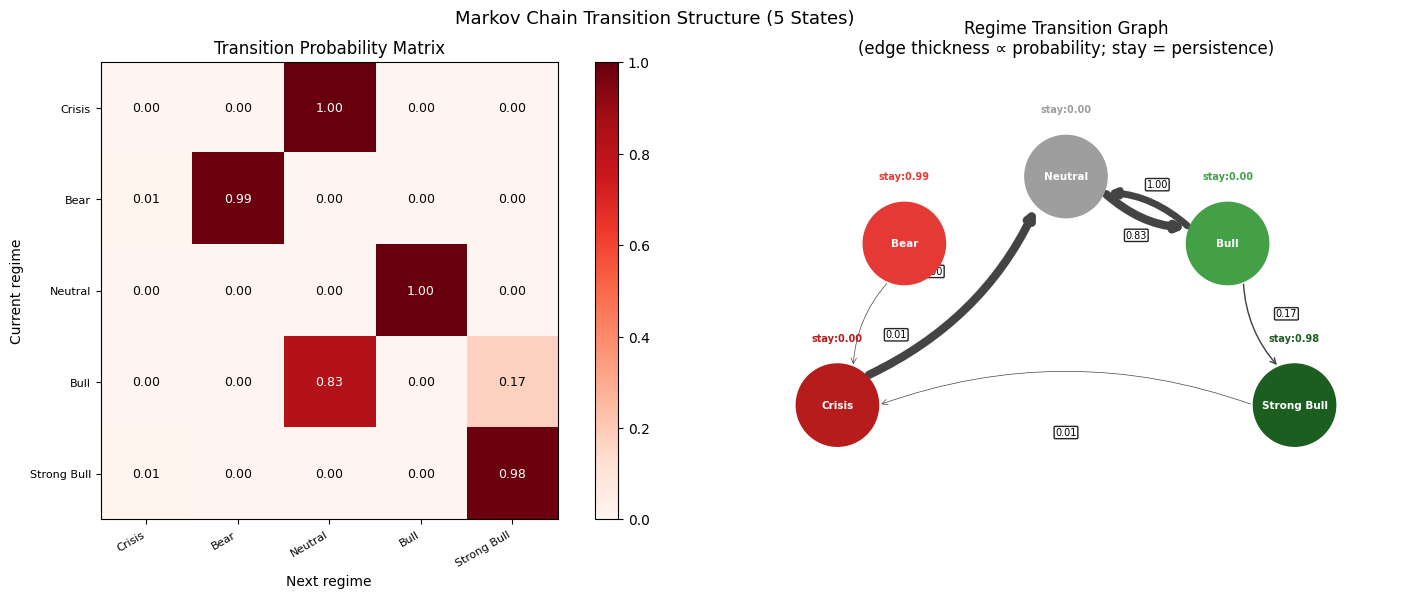
\includegraphics[width=0.95\linewidth]{images/hmmGraph.png}
    \caption{Regime changes with HMM. Regimes are much more persistent and less noisy}
    \label{fig:placeholder}
\end{figure}

\begin{figure}[h!]
    \centering
    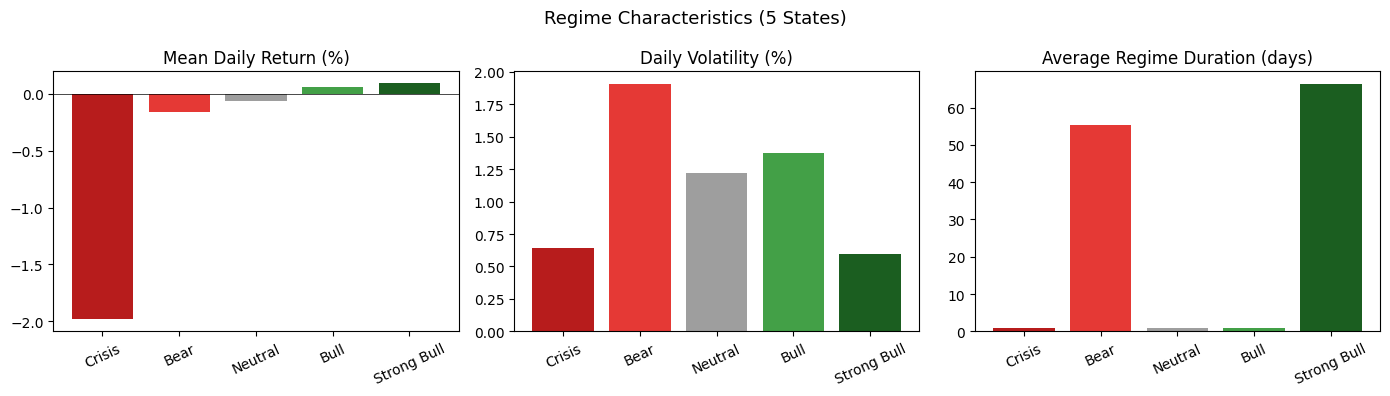
\includegraphics[width=1\linewidth]{images/RegimeCharactersitcs.png}
    \caption{Regime Characteristics}
    \label{fig:placeholder}
\end{figure}
\subsection{Prompt 3 - Graph Algorithm}
We now need a `decoding' algorithm - something that finds the single most likely sequence of hidden regime states given observed returns. 

\subsubsection{Prompt}
``We've trained a 5-state Gaussian HMM on S\&P 500 daily returns, where each hidden state represents a market regime. Now, given a new sequence of T observed daily returns, we want want to find the single most likely sequence of hidden regimes that produced those observations. Apply a graph algorithm/optimization to do this efficiently''.

\subsubsection{Response}
The Viterbi algorithm finds the most likely sequence of hidden states given a sequence of observations in a Hidden Markov Model. It works by dynamic programming:

\paragraph{Initialization}
For each state $s$, compute the probability of starting in $s$ and emitting the first observation:
\[
\delta_1(s) = \pi_s \cdot b_s(o_1)
\]

\paragraph{Recursion}
At each time step $t$, for each state $j$, find the best predecessor:
\[
\delta_t(j) = \max_i \left[ \delta_{t-1}(i) \cdot a_{ij} \right] \cdot b_j(o_t)
\]
where $a_{ij}$ is the transition probability from state $i$ to $j$, and $b_j(o_t)$ is the emission probability. Store the $\arg\max$ as a backpointer.

\paragraph{Termination}
Pick the state with the highest $\delta_T$ at the final time step.

\paragraph{Backtracking}
Follow backpointers to recover the full optimal state sequence.

\paragraph{Complexity}
This reduces complexity from $O(K^T)$ (brute-force over all state sequences) to $O(K^2 \cdot T)$, where $K$ is the number of states and $T$ is the sequence length. In your notebook, $K = 5$ and $T \approx 2{,}200$ trading days, so Viterbi evaluates $\sim 55{,}000$ operations instead of $5^{2200}$. 

\subsubsection{Evaluation}
We initially deemed the Viterbi Algorithm to be a suitable approach, having checked several academic sources on Hidden Markov Models (\cite{jurafsky2026}\cite{rabiner1989}). To transform the Virtebi algorithm into a tradeable strategy, we can mask each regime label with a position scalar. For example, we will be fully long in the Strong Bull case, flat in the Neutral case, and fully short in the Crisis case. The positions were much more stable (Figure 27) compared to the simple Markov chain (Figure 25) \\

\begin{figure}
    \centering
    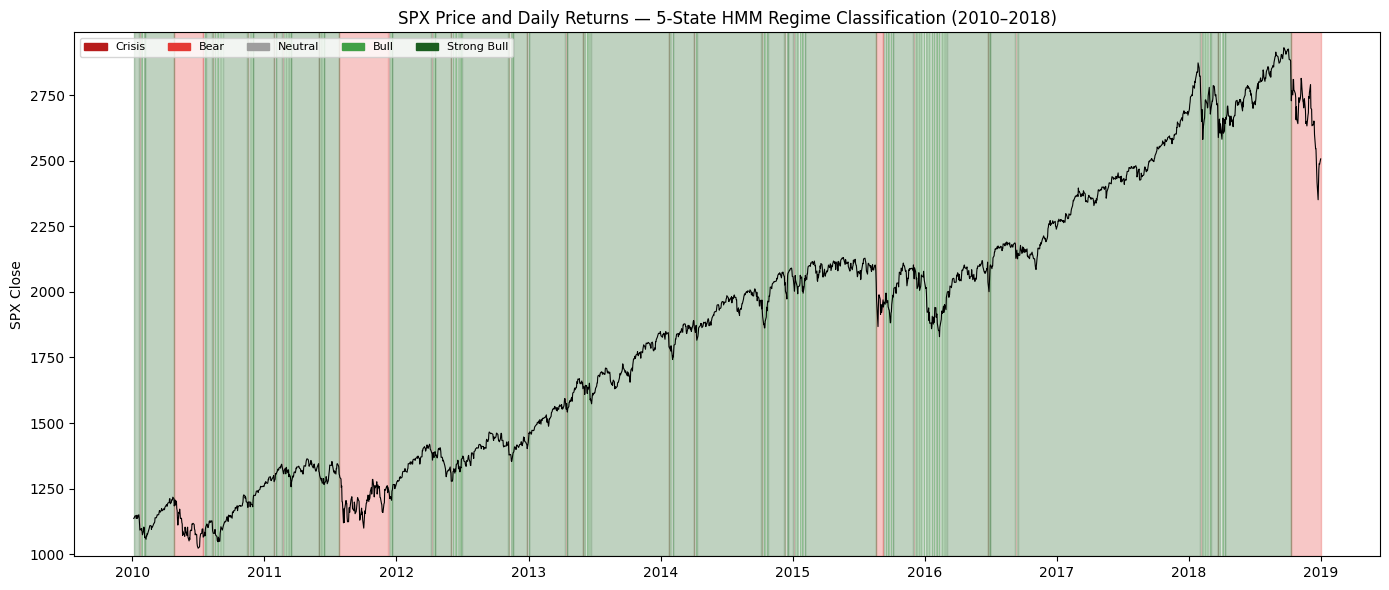
\includegraphics[width=0.95\linewidth]{images/HMMpositions.png}
    \caption{Training set regime labels using Viterbi}
    \label{fig:placeholder}
\end{figure}

However we later realized a key flaw in the LLM suggestion. Viterbi's backtracking step is the culprit. The backpointers are resolved \emph{backwards} from time $T$, meaning the regime label assigned to day $t$ implicitly conditions on all future observations $o_{t+1}, \ldots, o_T$. In a live trading context this is pure lookahead bias --- you are making decisions on January 3rd using information that only becomes available in March.

This is acceptable for post-hoc regime labelling on the training set (e.g., annotating historical data for analysis), but it is not a viable strategy on the test set, where you must act at time $t$ knowing only $o_1, \ldots, o_t$.

\subsection{Prompt 4 - Feed Forward Algorithm}

\subsubsection{Prompt}
``Explain how to replace the Viterbi algorithm with a causal alternative suitable for live trading.''

\subsubsection{Response}
``Replace Viterbi with the Forward algorithm, which computes the filtered state distribution --- the probability of being in each regime given only the information available up to and including the current day:
\[
\alpha_t(j) = P(s_t = j \mid o_1, o_2, \ldots, o_t)
\]

\textbf{1. Predict} (propagate yesterday's distribution forward through the transition matrix):
\[
\hat{\alpha}_t(j) = \sum_{i=1}^{K} \alpha_{t-1}(i) \cdot a_{ij}
\]

\textbf{2. Update} (weight by today's emission likelihood and normalise):
\[
\alpha_t(j) = \frac{\hat{\alpha}_t(j) \cdot b_j(o_t)}{\sum_{k=1}^{K} \hat{\alpha}_t(k) \cdot b_k(o_t)}
\]

The normalisation constant in the denominator ensures the distribution sums to one:
\[
P(o_t \mid o_1, \ldots, o_{t-1})
\]''

\subsubsection{Evaluation}
Unlike Viterbi, which produces a single most likely path using future information, the Forward algorithm does indeed maintain a full probability distribution over regimes. It is a strictly causal computation. This introduces some noise compared to the smoothed Viterbi path, but avoids lookahead bias and provides a principled basis for real-time decision-making (e.g., probabilistic position sizing or regime-based thresholds). Using the algorithms signals on the whole S\&P500, we apply these to trade 10 individual stocks:
\begin{table}[h!]
\centering
\begin{tabular}{lcccc}
\hline
\textbf{Ticker} & \textbf{Strategy Sharpe} & \textbf{B\&H Sharpe} & \textbf{Strategy Return (\%)} & \textbf{B\&H Return (\%)} \\
\hline
AAPL & 2.916 & 2.420 & 102.851 & 88.742 \\
MSFT & 2.552 & 2.322 & 58.413 & 58.259 \\
JPM  & 3.036 & 1.991 & 65.423 & 44.751 \\
XOM  & 0.546 & 0.264 & 9.316 & 4.925 \\
JNJ  & 1.117 & 0.973 & 18.686 & 17.403 \\
PG   & 2.048 & 2.080 & 36.696 & 40.680 \\
BA   & 0.258 & 0.099 & 7.489 & 2.920 \\
GS   & 2.213 & 1.333 & 61.441 & 36.412 \\
AMZN & 0.990 & 0.804 & 23.474 & 20.057 \\
CVX  & 1.173 & 0.682 & 21.702 & 13.295 \\
\hline
\end{tabular}
\caption{Strategy vs Buy-and-Hold Performance Comparison}
\label{tab:strategy_vs_bh}
\end{table}
\begin{figure}
    \centering
    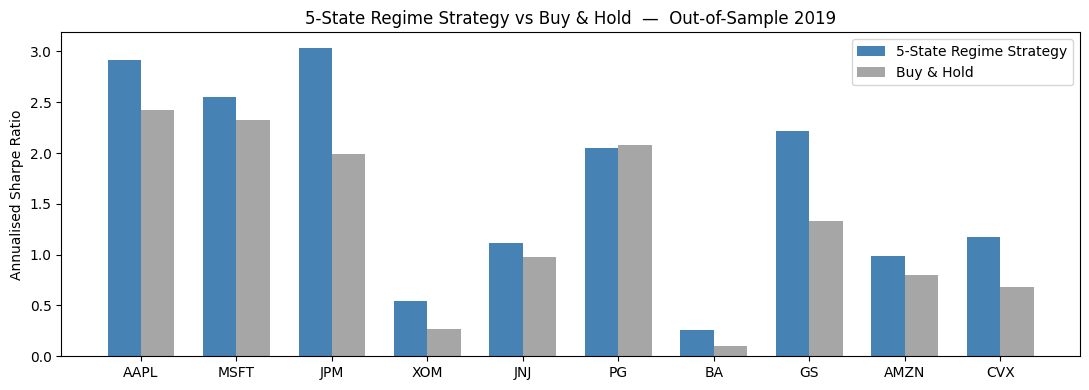
\includegraphics[width=0.95\linewidth]{images/singlestock.png}
    \caption{Forward filtering on individual stocks}
    \label{fig:placeholder}
\end{figure}
\clearpage
\subsection{Conclusion}

The study progressed through two distinct modelling stages. We started with a \textbf{simple (observable) Markov chain} by discretising S\&P 500 daily log-returns into $K$ quantile-based bins (Large Down through Large Up), counting transitions between bins, and treating the resulting row-stochastic transition matrix $\mathbf{P}$ as the weighted adjacency matrix of a directed graph. \\

An MDP was solved via value iteration to determine the optimal long/flat/short policy for each bin, and the strategy was evaluated out-of-sample.\\

The limitation of this approach is that discretisation boundaries are imposed by the analyst. Quantile bins are a reasonable heuristic, but they do not discover structure in the data. The bins therefore lack economic meaning and serve primarily as a statistical convenience.\\

This motivates the \textbf{Hidden Markov Model (HMM)}. The HMM treats the market regime as a \emph{latent} variable that cannot be directly observed. Each regime generates returns from its own Gaussian distribution, and the model infers the most likely sequence of hidden states from observed data.\\

\subsubsection{Connection to Deep Learning and Latent Variable Models}

This was an interesting study for us, as HMM fits into the broader framework of latent variable models used in COMP 60034 - Deep Learning. In both cases, observed data $\mathbf{x}$ is generated by unobserved latent variables $\mathbf{z}$.\\

In an HMM, the latent variable $z_t \in \{1, \dots, K\}$ represents the regime at time $t$. The emission model $p(\mathbf{x}_t \mid z_t)$ is typically Gaussian, and the transition model $p(z_t \mid z_{t-1})$ is a fixed matrix. Parameters are learned via Expectation-Maximisation (EM), alternating between inferring hidden states (E-step) and updating parameters (M-step).\\

A \textbf{Variational Autoencoder (VAE)} generalises this framework. The encoder $q_\phi(\mathbf{z} \mid \mathbf{x})$ approximates the posterior over latent variables, while the decoder $p_\theta(\mathbf{x} \mid \mathbf{z})$ models the data generation process. Training maximises the Evidence Lower Bound (ELBO).



Given a trained HMM and observed returns $(r_1, \dots, r_T)$, the \textbf{Viterbi algorithm} computes the most likely hidden state sequence:
\[
\hat{z}_{1:T} = \arg\max_{z_{1:T}} \; p(z_{1:T} \mid r_{1:T}).
\]

A brute-force approach requires evaluating $K^T$ paths, which is computationally infeasible. Viterbi solves this via dynamic programming:
\[
\delta_t(j) = \max_i \left[\delta_{t-1}(i) \cdot a_{ij}\right] \cdot b_j(r_t),
\]
where $a_{ij}$ are transition probabilities and $b_j(r_t)$ are emission probabilities.\\

\subsubsection{Evaluation \& Future Work}
Results showed that 9 out of 10 stocks achieved higher Sharpe ratios than buy-and-hold. The improvement was driven primarily by \textbf{volatility reduction}, as the model reduced exposure during high-volatility periods. The exception (BA) highlights a limitation: the regime signal is derived from index-level dynamics and may not capture firm-specific events.\\

In practice, we probably wouldn't use the HMM directly as a trading strategy. Instead one could feed these discovered regime features ( duration, type etc.) into a larger model (XGBoost, LSTM, etc.) alongside other standard price/volume features. 


\clearpage
\printbibliography
\end{document}